%===========================================================================
%	V. Implementation
%===========================================================================

This chapter accompanies the process of practical implementation of the target solution. It aims to enhance the current solution by means of the task definition (cf. Section \ref{sec:1-task}) and the findings from the actual state analysis (cf. Chapter \ref{chap:actual-state-analysis}). Specifically, three main aspects are expected to be added to the solution after implementation, being

\begin{enumerate}
	\item the decapsulation of the analytical scripts from the Apache Airflow instance,
	\item the inclusion of technical DataOps standards, specifically \acs{iam}, \ac{vcs}, \ac{cicd} and \ac{iac}, and finally
	\item the implementation of the DataOps testing framework (cf. Chapter \ref{chap:testing-framework}).
\end{enumerate}

The order of documentation does not necessarily reflect the implementation sequence of the project. Since this thesis can also be seen as a guideline for future DataOps projects, the implementation steps are provided in order to build on one another in the most useful way. The first two implementation tasks are performed for the entire data pipeline, while DataOps testing is exemplarily implemented for the Conversion Stage.

\section{Server-Less Architecture Enablement}
In order to achieve the goal of a (close-to) server-less architecture, the current architecture of the Value Pipeline needs to be revisited. Currently, the analysis is directly performed on the Airflow server instance (cf. Section \ref{sec:3-data-pipeline}). Instead, it is desired that each analytical step can be performed and configured independently while also complying to the server-less philosophy. This results in a high-level design change depicted in Figure \ref{fig:5-new-pipeline}.
\newpage

\begin{figure}[h!]
	\centering
	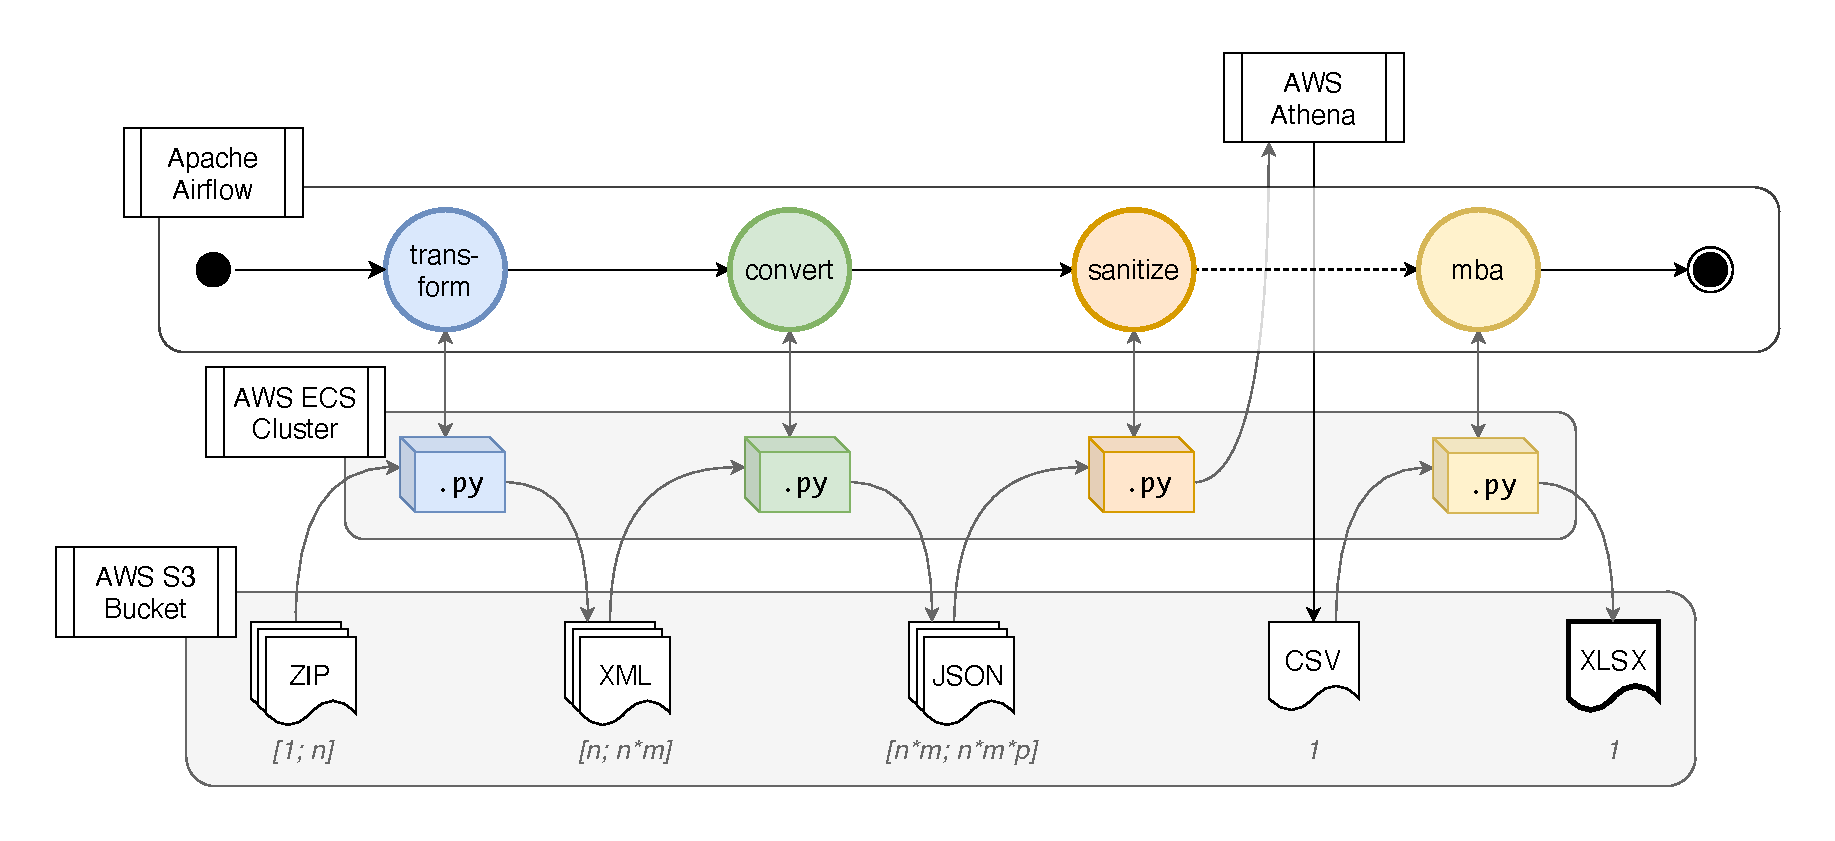
\includegraphics[width=\linewidth]{main-matter/img/5-new-pipeline.pdf}
	\caption{Revisited Data Pipeline Architecture (Server-Less)}
	\label{fig:5-new-pipeline}
\end{figure}

As visualized above, the new architecture outsources the Python analysis scripts outside of the Airflow instance. Instead, they new create individual microservices, deployed as virtual containers. These containers, typically realized with the \textit{Docker} containerization software \cite{docker}, contain all required dependencies to run their services. \ac{aws}' \textit{\ac{ecs}} can be used for the server-less deployment and execution of these container tasks \cite{ecs}. With this architecture change, Airflow only remains an orchestration tool that starts the appropriate container tasks. The tasks report their statuses back to Airflow, resulting in Airflow either triggering the next service or terminating the process if an error occurs.

\subsection{Microservice Containerization}
In microservice virtualization, containers are the final desired product. The goal is to have a sequence of commands that encapsulate the Python program code of each individual stage inside their own containers, considering individual stage requirements. To achieve this goal, the intermediate creation of a so-called \textit{image} is required, which provides basic components for making the service runnable \cite{docker}. Before running the container, specific configurations after the image has been defined.

Docker images are defined by means of a \textit{Dockerfile} \cite{docker}. The tasks inside this file are sequentially executed when creating the image. Exemplarily, the Dockerfile of the Conversion Stage can be seen below.
\newpage
\begin{listing}
	\inputminted{dockerfile}{main-matter/src/5-convert-dockerfile}
	\caption{Dockerfile of the Conversion Stage}
	\label{src:5-convert-dockerfile}
\end{listing}

As can be seen in Source Code Excerpt \ref{src:5-convert-dockerfile}, the image definition begins with referencing the base image (l. 1). This contains a slimmed-down operating system with the capability of running Python. The Dockerfile also specifies the working directory (l. 2) and prepares environment variables (ll. 4--11) for the container that contain \ac{aws} credentials as well as designated \ac{s3} path \acp{uri} for input and output data locations. The credentials are required for the service to perform its steps on the designated \ac{aws} infrastructure. These environment variables will receive their values during the build process of the container (i.e., when executing the image). Finally, the local package directory is added to the working directory of the image (l. 16) and all required Python dependencies (for both running and testing) are installed via the \acs{pip} Python package manager (ll. 18--19). These dependencies are specified in the applicable \texttt{requirements.txt} files inside the package directory.

The environment variables will prove valuable during DataOps enablement. By defining granular \ac{aws} credentials, each stage is only authorized to read and write to their designated \ac{s3} data lake subareas. This creates separated environments for each development stage.

The image can now be build using the \texttt{docker build} command. The design of the Dockerfile requires that the environment variables are passed before container execution (i.e., via arguments in the \texttt{docker build} or \texttt{docker run} command). The image receives a unique tag and the Dockerfile is referenced for correct handling of relative paths. Finally, the image can be used for running the container. This is achieved using the \texttt{docker run} command, specifying which command to run inside the container (e.g., for the Conversion Stage, \texttt{python ./convert.py} for executing the analytics script). This runs the container inside the local system.

\subsection{Image Deployment}
Instead of the container running locally, it is desired to execute it inside the server-less \ac{ecs}. This requires the preliminary deployment to an associated \ac{aws} service, the \ac{ecr}. \ac{ecr} is an image repository that is designed to hold different versions of an image \cite{ecr}. The image deployment and container execution strategy is depicted in Figure \ref{fig:5-container-deployment} below.

\begin{figure}[h!]
	\centering
	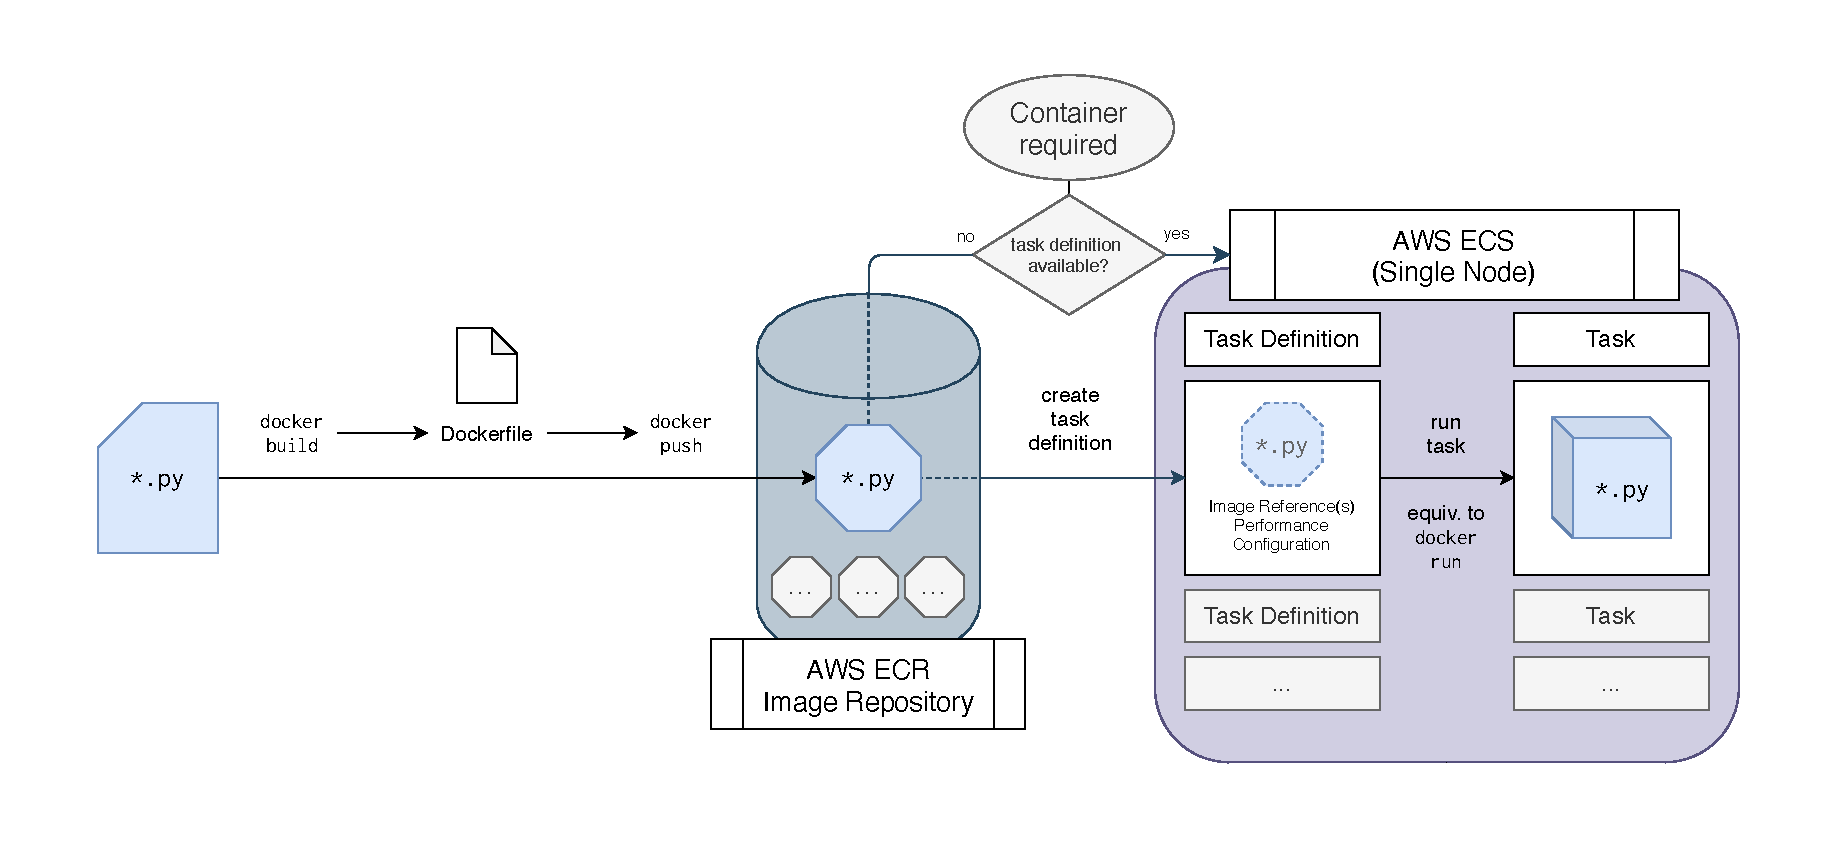
\includegraphics[width=\linewidth]{main-matter/img/5-container-deployment.pdf}
	\caption{Microservice Deployment Process}
	\label{fig:5-container-deployment}	
\end{figure}

Following the flow of the figure, the image is build by means of its Dockerfile and pushed to the designated \ac{ecr}. The octagon shape is used to describe an image. The execution requires another preliminary step which is the task definition of the container. This is because \ac{ecs} can also perform container execution sequences, periodic repetitions of the task, etc. Plus, each task can have different performance requirements. The task definition allows for individual hardware specification (e.g., processing power, memory, etc.) \cite{ecs}. Thus, the task definition can be seen as a blueprint for the (more or less complex) container service. For the data pipeline stages, a task with basic performance specifications as well as one image reference for running the applicable container once, suffices. The task can now be run based on its task definition, providing information on which Python script to run. This executes the task and tears down the container after the task has been worked through or an error has occurred. When the container service is required again and the image repository has not changed, the previous task definition can be directly executed.

\subsection{Server-Less Container Execution via Airflow}
Returning to the high-level overview, creating and running the task definition is performed by Airflow through the \ac{aws} Python \acs{api}, \texttt{boto3}. The Airflow \ac{dag} controller is redesigned to constantly evaluate the state of \ac{ecr} and \ac{ecs}. It checks for images inside each stage's image repository and builds the applicable task definitions. When all task definitions of all four pipeline stages are present, the Airflow \ac{dag} is ready for execution. The only task inside each individual step of the \ac{dag} is to execute the task definition and evaluating the container response.

Because of the periodic review, the most recent images and task definitions need to be saved inside Airflow variables to prevent the system to constantly recreate the same task definitions, resulting in an endless loop and, thus, in infrastructure overload.

In case a new version for a stage is recognized, a new task definition is created and re-referenced inside the \ac{dag}, enabling automatic updating of the pipeline solution.

\section{DataOps Enablement}
The next step is to include DataOps-related technologies to the project. They have mostly to do with general solution automation and environment management. Specifically, the following aspects are implemented and configured:

\begin{enumerate}
	\item Enhanced permission management via \acs{aws} \acf{iam},
	\item \acf{vcs} by using \textit{Git} and a \textit{GitHub} repository,
	\item \acf{cicd} by using the \textit{Jenkins} automation software, and
	\item \acf{iac} by using the \textit{Terraform} infrastructure automation tool as well as the \textit{Ansible} infrastructure provisioning software.
\end{enumerate}

These processes will support and build on each other during development for both automation and environment management disciplines.

\subsection{Enhanced Permission Management: \acs{aws} \acs{iam} Roles}
\acs{aws} \acs{iam} roles are used to provide different access permissions to different users and resources. If a user or resource tries to perform actions on \ac{aws} services (e.g., via \acs{cli} or \acs{api}), the system checks if the required credentials are present to perform this action. The credentials are provided in the form of asynchronous encryption, resulting in a public \textit{Access Key ID} and in a private \textit{Secret Access Key} \cite{iam}.

Because of the static nature of the current solution, only one full-access \ac{iam} role is used. This is not desirable from multiple perspectives. Each developer should be provided an \ac{iam} role that is sufficient for his or her needs. The underlying permissions should not exceed these needs in order to prevent collision or changes within \ac{aws} resources outside of the scope of the developer. The same aspect applies to resources that automatically perform actions on other resources. Another important factor is data privacy. In a production-grade environment with sensitive data, it is crucial and binding by law that the data is only seen and processed by authorized entities. 

For instance, if a data pipeline stage is misconfigured and tries to read from another area of the \ac{s3} data lake, the process will terminate when the given \ac{iam} role prohibits this action. Otherwise, the stage is granted access to data that is not required for its task. In that case, correctly configured \ac{iam} roles can also prevent errors in case the content of the incorrect \ac{s3} area cannot be processed by the current analytics stage.

Considering the \ac{mba} data pipeline, the present variety of resources requires different permissions on a number of other different resources. Table \ref{tab:5-iam} below describes all permissions required by different components.

\begin{table}[h!]
	\centering
	\begin{tabular}{r!{\vrule width 1pt}l|l|l}
\textbf{Component}                                  & \textbf{Resource}         & \textbf{Type} & \textbf{Scope}              \\ \ChangeRT{1pt}
\multirow{2}{*}{Airflow}                            & \ac{ecr} & Full Access   & designated stage image repositories          \\ \cline{2-4}
                                                    & \ac{ecs} & Full Access   & designated container cluster                 \\	 \ChangeRT{1pt}
\multicolumn{4}{c}{\textbf{Stages}}                                                                                           \\ \ChangeRT{1pt}
\multirow{2}{*}{\textbf{Transformation}}            & \ac{s3}  & Read          & \texttt{prod/landing/}      				  \\ \cline{2-4}
                                                    & \ac{s3}  & Write         & \texttt{prod/**/raw/}       				  \\ \hline
\multirow{2}{*}{\textbf{Conversion}}                & \ac{s3}  & Read          & \texttt{prod/**/raw/}       			  	  \\ \cline{2-4}
                                                    & \ac{s3}  & Write         & \texttt{prod/**/converted/} 				  \\ \hline
\multirow{3}{*}{\textbf{Sanitization}}              & Athena   & Full Access   & designated database                          \\ \cline{2-4}
                                                    & \ac{s3}  & Read          & \texttt{prod/**/converted/} 				  \\ \cline{2-4}
                                                    & \ac{s3}  & Write         & \texttt{prod/**/sanitized/} 				  \\ \hline
\multirow{2}{*}{\textbf{\ac{mba}}} 					& \ac{s3}  & Read          & \texttt{prod/**/sanitized/}  				  \\ \cline{2-4}
                                                    & \ac{s3}  & Write         & \texttt{prod/**/}          
\end{tabular}
	\caption{\acs{aws} \acs{iam} Role Overview}
	\label{tab:5-iam}
\end{table}

These roles are setup within the \ac{aws} \ac{iam} Console and passed to the individual components as environment variables \cite{iam}, depending on their individual deployment. 

\subsection{\acs{vcs} Enablement: \textit{Git} and \textit{GitHub}}
Embedding the project inside a \ac{vcs} allows for collaborative development. When working with such a system, the common codebase is located inside a distributed repository. This repository can be cloned (i.e., copied) to the developers local development environment. \textit{Committing} (i.e., performing and saving changes of the personal version of ones source code) does not collide with the source code versions of other developers \cite[9\psqq]{Chacon2020}. Plus, since the project at hand relies on external programming and developing dependencies (e.g., Python packages and libraries, environment configuration processes, etc.), the repository can also contain configuration utilities for setting up the developing sandbox.

\subsubsection{Repository Structure}
A cloned repository is a typical project directory. The repository for the \ac{mba} data pipeline solution looks as follows:

\begin{figure}[h!]
	\centering
	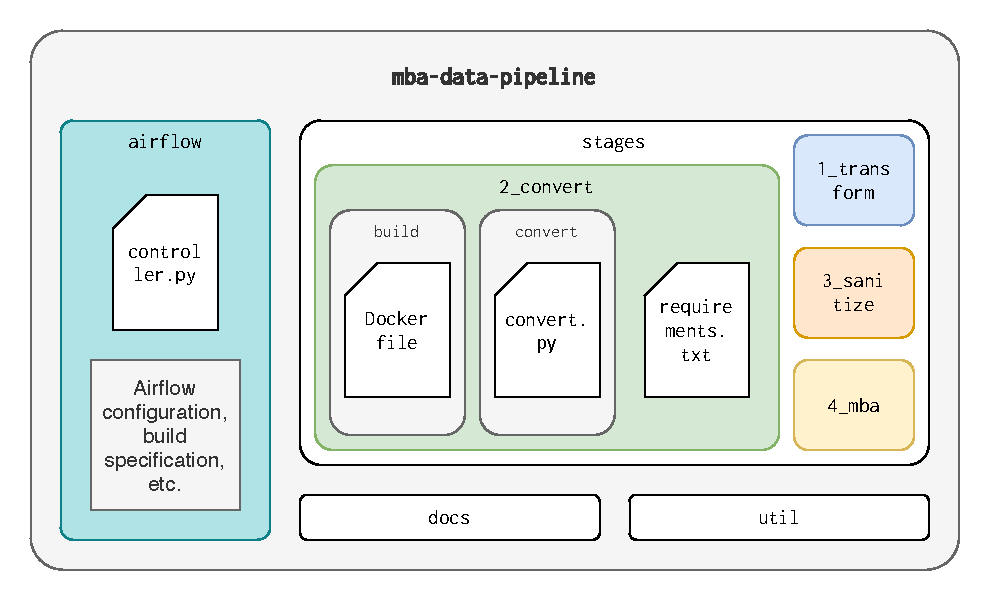
\includegraphics[width=\linewidth]{main-matter/img/5-repo-structure.pdf}
	\caption{Initial Project Repository Structure}
	\label{fig:5-repo-structure}
\end{figure}

The repository presented in Figure \ref{fig:5-repo-structure} is a so-called \textit{monolithic} repository. Since the project is expected to be developed by separate stage teams, this repository de facto consists of multiple projects. Starting at the root of the directory, the repository contains subdirectories for Airflow pipeline management, the individual stages of the data pipeline, documentation as well as miscellaneous utilities. The Airflow pipeline management consists of the pipeline controller script, as well as supporting build files that are outside the scope of this thesis. More importantly, the individual stages are, again, divided into subdirectories. Each stage has its own build directory (currently including its Dockerfile), a package directory (currently including all productive source code), as well as dedicated requirements files required by the source code).

\subsubsection{Repository Setup}
The goal is to create a GitHub repository for the \ac{mba} data pipeline project. First, the project needs to become a Git repository, enabling the version control capability. GitHub is used for the distribution and collaborative management of the code base \cite[25\psqq]{Chacon2020}\cite{github}. First, the project directory needs to be initialized by means of Git. Then, the repository can be created within the GitHub web \ac{ui}. Lastly, the local Git repository is pushed to the recently created GitHub repository.

In order to allow for the automatic configuration of development sandboxes, each stage directory receives a \textit{Makefile} that creates shortcuts for configuration commands. This includes local building and executing of a Docker container. Other development conventions (e.g., for Python, that development should be conducted in Python \textit{virtual environments}), cannot be enforced but only suggested within the project documentation.

\subsubsection{Branching Strategy}
Currently, an authorized developer is able to clone this repository, make any kind of changes, and push the changes back to the repository. This kind of workflow is not desired which is why \textit{branching} is introduced. Branching is a GitHub feature that supports development environment management within the repository \cite[62\psqq]{Chacon2020}. At this point, only one branch, the \texttt{master} branch, exists. It holds the history of all versions of the source code. These versions change when updated code is pushed to the brach. In practice, the \texttt{master} branch is supposed to be the communal \textit{single version of the truth}. It is expected to be runnable and should reflect the source code of the solution which is currently used in production. When changes of all sorts are possible inside the \texttt{master} branch, the validity of it gets lost. This is why this branch needs to be protected such that only evaluated changes can be pushed to this area of the repository.

Branching is a matter of project convention definition. The general goal is that on-going development of an arbitrary feature is conducted outside of the \texttt{master} branch (i.e., on separated feature branches). Each (sub-)team working on an individual feature \textit{branches} from the \texttt{master} branch, resulting in an exact copy of its origin in the beginning. All changes pushed to the new branch do not affect the \textit{master} brach. When the feature is considered done, a GitHub \textit{pull request} is created \cite{github}. This pull request is evaluated based on its configuration. If the evaluation passes, the feature branch gets \textit{merged} with the \texttt{master} branch, meaning that all changes are applied to the source code inside the \texttt{master} branch at once. Finally, the feature branch is deleted. From now on, the updated \texttt{master} branch is used as the starting point for further development. This branching workflow is commonly referred to as the \textit{GitHub Flow} \cite{GitHub2020}, depicted in Figure \ref{fig:5-github-flow}, below.

\begin{figure}[h!]
	\centering
	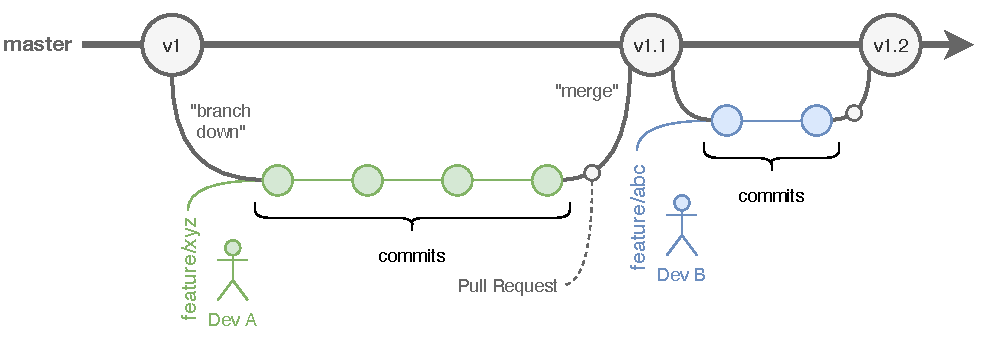
\includegraphics[width=\linewidth]{main-matter/img/5-github-flow.pdf}
	\caption[\textit{GitHub Flow} Branching Strategy]{\textit{GitHub Flow} Branching Strategy (per \cite{GitHub2020})}
	\label{fig:5-github-flow}
\end{figure}

The branching strategy, as presented above, is typical for a fast-paced development cycle. Each approved change, no matter how small, is directly published into production. Apart from that, other branching strategies could be applied. It might be reasonable to include separate \texttt{development} and \texttt{release} branches. The \texttt{development} branch could become the starting point for new features and could contain features that have not been published yet. In case of a slower release cycle, the development branch could be merged with the \textit{release} branch for compatibility testing purposes and deployed into production (i.e., merged with the \texttt{master} branch) afterwards. Another \texttt{hotfix} branch might be used for quick bug fixes that branches from the \textit{master} branch, fixes the bug, and merges back into production \cite{Driessen2010}.

For the sake of simplicity and demonstrability, the previously described branching strategy is chosen for the \ac{mba} data pipeline. The \texttt{master} branch is configured inside GitHub to only accept pull requests for incoming changes, not direct pushed onto the \texttt{master} branch. Later, the pull request functionality will be enriched with \ac{cicd}. In case the process runs through without errors, the changes are evaluated positively and cleared for the merging process.

\subsection{\acs{cicd} Enablement: \textit{Jenkins}}
\ac{cicd} is expected to enhance and automate two aspects inside the development process of the \ac{mba} data pipeline solution:
\begin{enumerate}
	\item It handles the build and deployment of virtual Docker images and containers by means of Figure \ref{fig:5-container-deployment}. This also includes providing each task with its designated environment variables for infrastructure access as well as analysis data input and output locations.
	\item It automates the execution and reporting of test cases, only allowing for approved deployment of tested versions of the solution. This process supports the previously mentioned pull requests which will fail when tests are evaluated negatively.
\end{enumerate}

The latter aspect will be implemented in Section \ref{sec:5-testing-implementation}.

The desired DataOps \ac{cicd} workflow is depicted in Figure \ref{fig:5-cicd}. It considers testing a black box for now. It is noteworthy to mention that each stage of the data pipeline could have different requirements for its deployment, which is why each stage receives its own \ac{cicd} pipeline. This becomes clear when considering testing since each stage performs different tasks and requires different test cases.

\begin{figure}[h!]
	\centering
	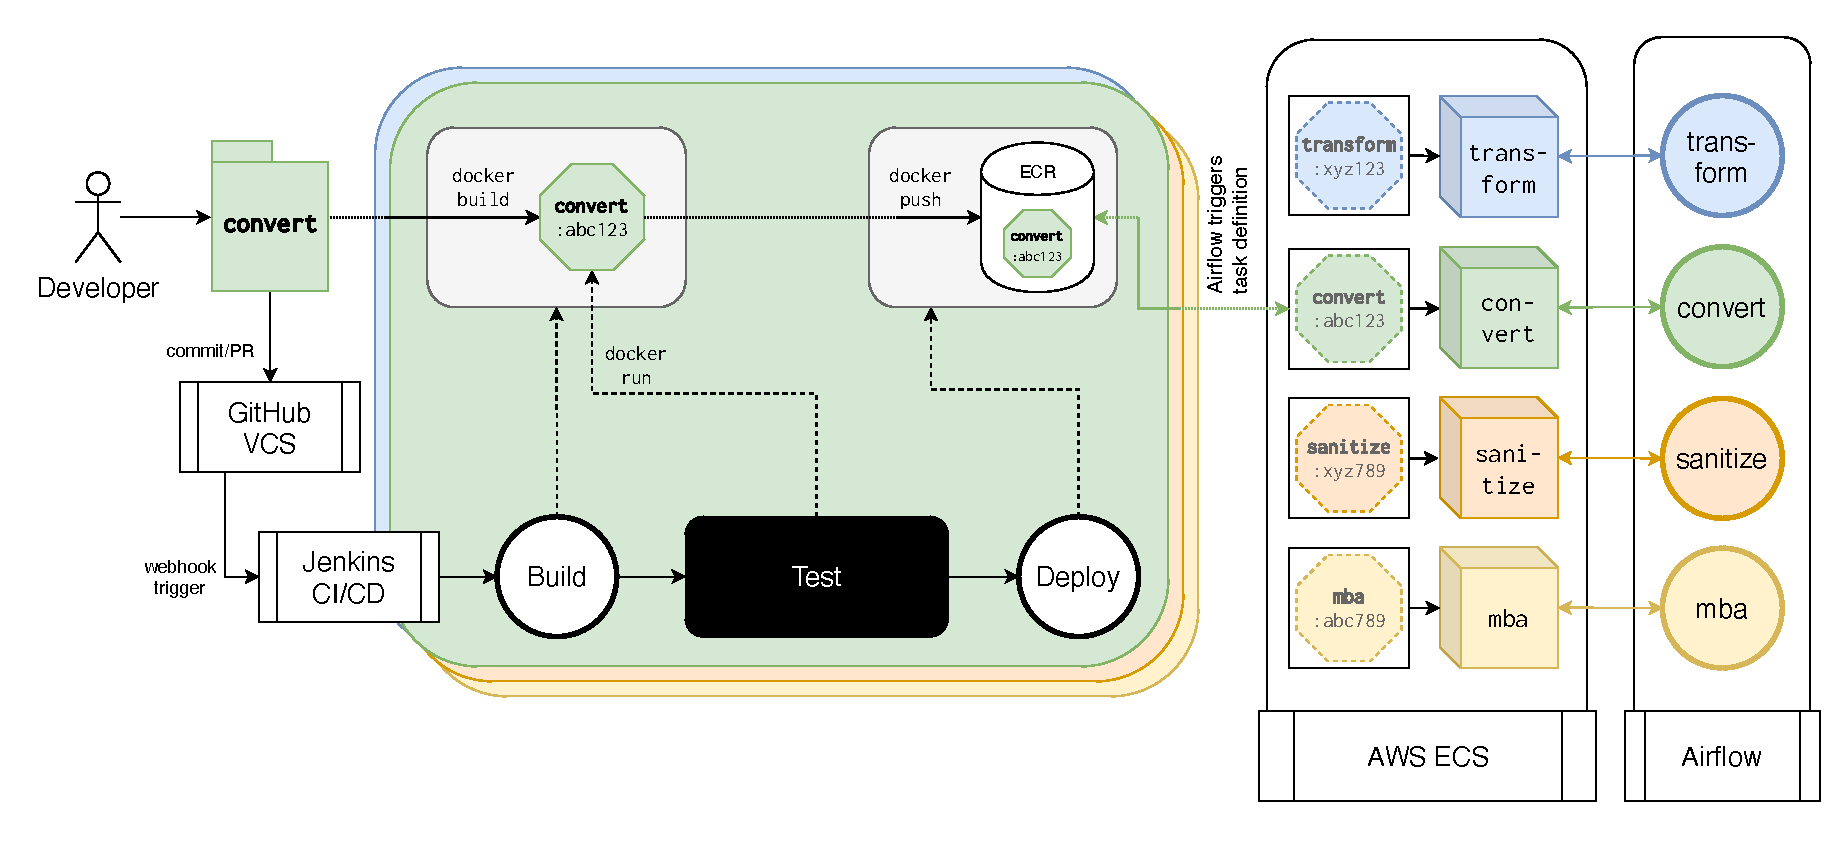
\includegraphics[width=\linewidth]{main-matter/img/5-cicd.pdf}
	\caption{DataOps \acs{cicd} Architecture for the Conversion Stage}
	\label{fig:5-cicd}
\end{figure}

Figure \ref{fig:5-cicd} represents the \ac{cicd} workflow of the Conversion Stage. It is meant to be executed whenever a GitHub pull request of a Convert Stage-related feature is opened. This pull request appearance should trigger the corresponding pipeline, realized with the \textit{Jenkins} \ac{cicd} software \cite{jenkins}. The first step needs to build a virtual Docker image using the target source code files from the pull request. Again, this build process is done by means of the stage's specific Dockerfile and requires additional arguments for the containers environment variables. When the image is built, the build stage of the \ac{cicd} pipeline is completed. Later, this this image will be run on the Jenkins instance for different testing purposes. After these tests pass, the image is ready for deployment. Airflow expects runnable images inside their designated \ac{ecr} repositories which is why the image, individually tagged, is pushed to its repository. The deployment process is done at this point. When Airflow needs to run a new analysis, the controller script will scan the registry for the latest image, recognize a new image, create the applicable task definition and run the container based on the newly deployed image. Every further analysis will be done utilizing this image until a new image is deployed again.

\subsubsection{Jenkins Software and Pipeline Setup}
Comparable to Apache Airflow, Jenkins needs to be considered as an external application that needs to reside on some kind of infrastructure. For efficiency reasons, the \ac{ec2} instance already running Airflow also receives Jenkins. Both web servers now run simultaneously on different ports for \acs{http} access.

Jenkins provides different blueprints for \ac{cicd} pipelines. The DataOps \ac{cicd} pipeline of the \ac{mba} data pipeline needs to recognize pull requests that originate from different feature branches within GitHub. This is why the \textit{Multibranch Pipeline} is chosen \cite{jenkins}. Such a pipeline is created for each of the four stages of the data pipeline. The branch needs to be granted access to the GitHub repository. Since the project is working with a monolithic repository, each \ac{cicd} pipeline needs to be configured in such a way that it only recognized changes and pull requests to specific areas of the repository.

There are multiple ways to achieve this configuration. Jenkins distinguished between branches and pull requests, meaning that a branch with a pending pull request is listed and evaluated by Jenkins \textit{twice}. Jenkins is therefore configured to disregard branches that are also filed as pull requests. The only non-pull request branch should be the \texttt{master} brach since all other branches are expected to be in development if no pull request is present. Thus, Jenkins should only consider \texttt{master} a long-lasting branch. The pipeline should only consider stage-specific changes, which is why Jenkins should filter each pull request by its GitHub label. This requires the developer to add the specific labels when filing a pull request. Finally, Jenkins should automatically run a \ac{cicd} job inside the corresponding pipeline when a change is recognized. This needs to be enabled in both Jenkins and GitHub. GitHub needs to send a \texttt{POST} request to Jenkins when a pull request is filed, whereas Jenkins needs to trigger the corresponding pipeline on \texttt{POST} request arrival.

\subsubsection{Jenkins Credential Management}
The virtual microservices need to receive their \ac{aws} \ac{iam} access credentials during their build process. Since this process is expected to be covered by \ac{cicd}, Jenkins needs to hold these credentials and pass these to the corresponding stage containers inside its \ac{cicd} pipeline workflow. This is achieved by adding the individual credentials to Jenkins' encrypted credential storage \cite{jenkins}. These need to include all stage-related credential key-value pairs that provide appropriate access to the analytics resources as described in Table \ref{tab:5-iam}. Additionally, Jenkins needs to be granted permission to push images to the \ac{ecr} repositories. The corresponding credential should not be mistaken with a separate \ac{iam} role. Rather, Jenkins needs to hold a login token for \ac{ecr} that is retrieved via \ac{aws} \acs{cli} \cite{ecr}. This process is identical to other Docker registry services, independent from vendor.

Jenkins will then pass the encrypted credentials to the corresponding pipelines \cite{ecr}, resulting in no hard-coded credentials in any configuration file.

\subsubsection{Pipeline Workflow Declaration}
After the pipeline preferences have been configured, the actual pipeline workflow needs to be declared for each stage. In Jenkins, this is done via a so-called \textit{Jenkinsfile}. It is written in \textit{Groovy} programming language and contains instructions for each stage of the pipeline \cite{jenkins}. A sample Jenkinsfile for the Conversion Stage is shown below.
\newpage
\begin{listing}[h!]
	\inputminted{groovy}{main-matter/src/5-jenkinsfile-build}
	\caption{Jenkinsfile Build Stage for the Conversion Stage}
	\label{src:5-jenkinsfile-build}
\end{listing}

Source Code Excerpt \ref{src:5-jenkinsfile-build} shows the build stage inside the Jenkinsfile. It retrieves the corresponding stage credentials from Jenkins' credential storage (ll. 8--11) and executes the build process of the Docker image (ll. 12--19). The image needs to be tagged in an \ac{aws}-provided \ac{ecr} format such that it is assigned to the correct repository during the deployment phase. This tag includes the corresponding Git commit ID for versioning purposes (l. 14) which is passed to Jenkins by the previously mentioned GitHub \texttt{POST} request trigger. Prior to the build, the arguments for the \ac{aws} \ac{iam} credential pair are passed (ll. 15--16) and set as environment variables by means of the Dockerfile specification. Finally, the Dockerfile (l. 17) and the build context for relative path recognition (l. 18) are specified. This command is executed by the Jenkins \ac{cicd} pipeline job. In case of a correct execution, the next stage is performed. Since testing is omitted for now, it directly continues with the deployment, shown below. 
\newpage
\begin{listing}[h!]
	\inputminted{groovy}{main-matter/src/5-jenkinsfile-deploy}
	\caption{Jenkinsfile Deployment Stage for the Conversion Stage}
	\label{src:5-jenkinsfile-deploy}
\end{listing}

Source Code Excerpt \ref{src:5-jenkinsfile-deploy} shows the deployment stage inside the Jenkinsfile. It retrieves the \ac{ecr} credentials (ll. 11--13) and performs the image deployment via \texttt{docker push} (ll. 14--17). This action is performed for two tags: the commit ID for versioning and the conventional \texttt{latest} tag such that Airflow recognizes it as the most recent, production-ready image. \\\

All in all, the current \ac{cicd} solution builds and deploys a new version into production when a feature pull request is filed to GitHub. Airflow recognizes the change based on its controller script and uses the new image for the corresponding stage for container execution and evaluation.

\subsection{\acs{iac} Enablement: \textit{Terraform} and \textit{Ansible}}
Another form of automation that is part of DataOps is automatic infrastructure deployment via \ac{iac}. The project at hand requires a variety of different \ac{aws} infrastructural resources, including the effort of configuration. In case that the infrastructure needs to be setup inside a different \ac{aws} account or it breaks during development, it is not desirable to be forced to start building up the infrastructure from scratch. Instead, the following \ac{iac} architecture is proposed.

\begin{figure}
	\centering
	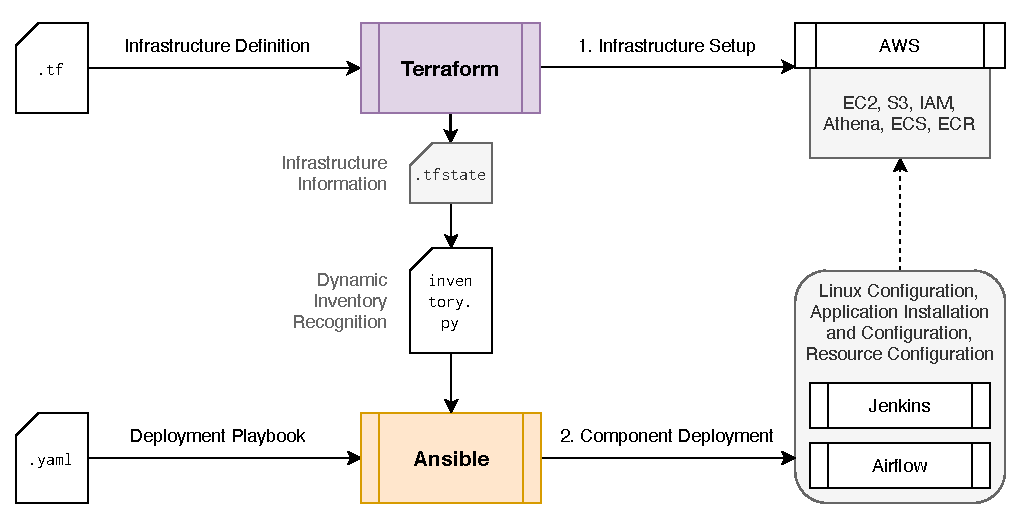
\includegraphics[width=\linewidth]{main-matter/img/5-iac}
	\caption{\acs{iac} Infrastructure Deployment Strategy}
	\label{fig:5-iac}
\end{figure}

The \ac{iac} architecture, visualized in Figure \ref{fig:5-iac}, is made out of two steps. First, all required \ac{aws} services are defined for the \textit{Terraform} infrastructure provisioning tool. This also includes basic configuration of networking and access management. In general, all configuration that can be done via the web \acs{ui}-based \ac{aws} Console or the \ac{aws} \acs{cli} or \acs{api} can be done via Terraform. Terraform requires an individual \ac{iam} role that allows it to create the infrastructure. When the deployment script is performed via the Terraform \acs{cli}, it creates a \texttt{.tfstate} file in \ac{json} format \cite{terraform}, summarizing all created infrastructure including public IP addresses, infrastructure IDs, etc.

This infrastructure needs to be configured via the \textit{Ansible} infrastructure orchestration software. This includes the Linux configuration of the \ac{ec2} instance, the creation of \ac{s3} data lake (sub-)areas, etc. Basically, the goal is to run the corresponding commands for Terraform and Ansible, resulting in an up-and-running infrastructure, ready for production-grade usage.

Ansible requires an intermediate step before being able to perform actions on the infrastructure, which is the recognition of the resource inventory. This can be done manually, which is not desired, or via a dynamic inventory recognition script. This makes use of the previously generated \texttt{.tfstate} file and provides Ansible with information and access to the respective infrastructure. Then, so-called Ansible \textit{Playbooks} are written and executed. These hold tasks for the configuration, platform and application installation, etc. \cite{ansible}. Most importantly, Ansible is in charge of installing and configuring Airflow and Jenkins. Airflow is installed and receives its controller script as well as further configuration from the project repository. Jenkins is installed, pre-configured, and required plugins are installed. 

Unfortunately, these applications do not provide all necessary Ansible endpoints. This means that not all configuration steps can be done automatically but require manual adjustment. This includes Jenkins credential management, pipeline creation, etc. All in all, the infrastructure automation is valuable nonetheless since the manual setup process is significantly reduced.

\section{Testing Framework Implementation} \label{sec:5-testing-implementation}


